% Evidence-Grounded Embodied Agents — Paper I (H1+H2)
% arXiv-ready skeleton. Compile: latexmk -pdf main.tex
% Results sections are deliberately marked PENDING: numbers must come from
% the frozen harness (see EXPERIMENT_DESIGN.md). No fabricated data.
\documentclass[11pt]{article}
\usepackage[margin=1in]{geometry}
\usepackage{amsmath,amssymb}
\usepackage{booktabs}
\usepackage{graphicx}
\usepackage{xcolor}
\usepackage{enumitem}
\usepackage[hidelinks]{hyperref}
\usepackage{tikz}
\usetikzlibrary{arrows.meta,positioning}

\newcommand{\pending}[1]{\textcolor{red}{[PENDING: #1]}}
\newcommand{\sys}{\textsc{AgenticWM}}

\title{\textbf{Evidence-Grounded Embodied Agents:\\
Transactional World Models and Continual Decision Learning\\
for Warehouse Robotics}\\
\large (Paper I: Physical-Evidence-Gated Transactions and Reliable Agentic Execution)}
\author{Guohongbin Xiang \and \pending{co-authors, affiliation}}
\date{\today}

\begin{document}
\maketitle

\begin{abstract}
LLM agents are increasingly proposed as orchestration layers for robotic fleets,
yet their acceptance in operational settings is blocked by a trust problem:
an agent can \emph{narrate} success without the physical world having
accomplished it. We present \sys{}, an agentic warehouse system in which
(a) business facts commit to a transactional world model \emph{only} when
sensor-derived physical evidence (support ratio, contact state, withdrawal
clearance) proves them; (b) the agent is the sole command entry but has no
capability to write facts; and (c) all execution runs on a contact-faithful
physics engine whose geometry is derived from a single versioned engineering
parameter source. We formalize five system invariants
(location conservation, evidence gating, agent write isolation, idempotency,
lease exclusivity) and describe a pre-registered evaluation protocol against
fair baselines, including fault-injection of forged, duplicated, delayed and
lost completion reports.
Results: H1 invalid-commit reduction is established by a 1{,}200-episode
fault-injection study (\S\ref{sec:h1}); \pending{H2 valid-completion-rate under escalating task complexity and disturbances}.
The system, physics tests (325 passing), and live demonstration interface are
publicly available.\footnote{\url{https://github.com/guohongbin-git/agv-world-model}}
\end{abstract}

\section{Introduction}
Robotic automation is usually sold as labor substitution. We argue, following
a line of evidence from cyber-physical systems, digital-twin, measurement-science
and data-flywheel literatures (Sec.~\ref{sec:related}), that its deeper value is
\emph{informational}: human execution produces deviations that are systematically
under-observed, so plans cannot be optimized against reality. An embodied agent
operating inside a transactional world model turns every physical action into
measurable, attributable, auditable evidence---but only if the system makes it
impossible to record what did not happen.

This paper takes the trust question literally: what happens when the agent
\emph{lies} (honestly or not) about execution? Our answer is an architecture in
which narration and fact are separated by a physics-verified commit gate.
Contributions:
\begin{enumerate}[label=C\arabic*.]
\item \textbf{Evidence-gated transactional execution.} A world model in which
every inventory mutation is a database transaction admitted only by a
sensor-evidence predicate evaluated on the physics state, with explicit
failure semantics (\texttt{CommitEvidenceMissing}) and Saga-style compensation
boundaries for the un-rollbackable physical world.
\item \textbf{Agent write isolation.} The LLM/rule agent is the only command
entry (task submission, pause, re-dispatch, queries) and provably holds no
fact-writing capability; observation channels are physically separated from
ground truth used only for evaluation.
\item \textbf{A pre-registered evaluation protocol} (Sec.~\ref{sec:protocol}):
four architecture variants sharing one execution kernel; fault-injection of
forged/duplicated/delayed/lost reports; statistical plan with clustered
confidence intervals; published seeds and harness for third-party replay.
\end{enumerate}

\section{Related Work}\label{sec:related}
\paragraph{World models.}
Ha \& Schmidhuber~\cite{ha2018world} introduced learned latent world models;
DreamerV3~\cite{hafner2023dreamerv3} learns control in imagination;
surveys~\cite{wu2024understanding} separate ``understanding'' from ``predicting''
camps. We take the classical control-theoretic reading: a world model is a
queryable, committable state machine over the physical world, not a video
generator.
\paragraph{LLM agents for robotics.}
SayCan~\cite{ahn2022saycan} grounds affordances; Code as Policies~\cite{liang2022cap};
Voyager~\cite{wang2023voyager} builds skill libraries in a simulator;
Reflexion~\cite{shinn2023reflexion} stores verbal feedback;
RAP~\cite{hao2023rap} and WALL-E~\cite{zhang2024walle} couple LLM search to
explicit world models. Our agent differs by the \emph{transactional} contract:
experience and intent may change plans, never facts.
\paragraph{Digital twins and execution intelligence.}
Tao et al.~\cite{tao2018dt}, Kritzinger~\cite{kritzinger2018dt} (digital model vs.\
shadow vs.\ twin), NIST measurement science for manufacturing
robotics~\cite{nist2024msr}, process mining~\cite{adriansyah2012replaying},
robot-powered data flywheels~\cite{grannen2025flywheel,yu2026logistics}.
LLM-agent-plus-twin systems appear in plant fault handling~\cite{bhalja2025llmdt}
and factory multi-agent control~\cite{gautam2025iiot}; none enforces
physics-evidence-gated business commits as we do.

\section{System}\label{sec:system}
\subsection{Architecture}
\begin{figure}[h]\centering
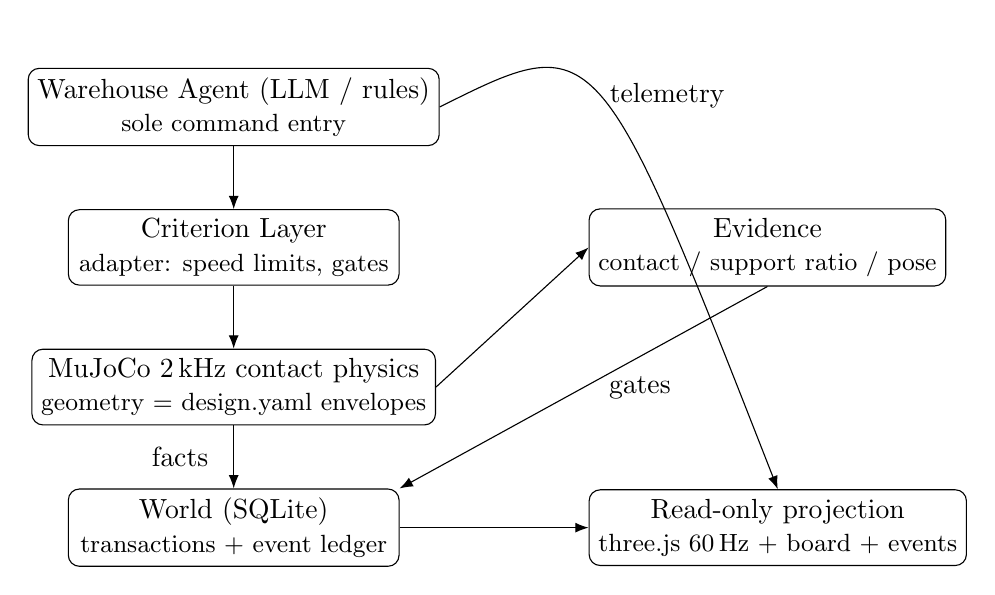
\begin{tikzpicture}[node distance=8mm,box/.style={draw,rounded corners,minimum width=42mm,minimum height=8mm,align=center}]
\node[box] (agent) {Warehouse Agent (LLM / rules)\\ \small sole command entry};
\node[box,below=of agent] (crit) {Criterion Layer\\ \small adapter: speed limits, gates};
\node[box,below=of crit] (phys) {MuJoCo 2\,kHz contact physics\\ \small geometry $=$ design.yaml envelopes};
\node[box,below=of phys] (world) {World (SQLite)\\ \small transactions + event ledger};
\node[box,right=24mm of crit] (obs) {Evidence\\ \small contact / support ratio / pose};
\node[box,right=24mm of world] (disp) {Read-only projection\\ \small three.js 60\,Hz + board + events};
\draw[-{Latex}] (agent) -- (crit);
\draw[-{Latex}] (crit) -- (phys);
\draw[-{Latex}] (phys) -- (world) node[midway,left,xshift=-2mm]{facts};
\draw[-{Latex}] (phys.east) -- (obs.west);
\draw[-{Latex}] (obs.south) -- (world.north east) node[midway,right,xshift=2mm]{gates};
\draw[-{Latex}] (world.east) -- (disp.west);
\draw[-{Latex}] (agent.east) .. controls +(2,1) .. node[right]{telemetry} (disp.north);
\end{tikzpicture}
\caption{\sys{}: intent flows down; facts flow up only through the evidence gate.}
\end{figure}

\subsection{Single parameter source}
All envelopes, speeds, thresholds derive from versioned
\texttt{configs/design.yaml}; the same geometry instantiates the MJCF collision
bodies, the criterion layer, and the photoreal visual meshes (offline renders
and the web twin are driven by the identical pose stream).

\subsection{Invariants}
Let $H(p)\in\{\text{SLOT:}s,\text{STATION:}h,\text{ROBOT:}r\}$ be a pallet's
committed holder and $\hat H(p)$ its physical support state estimated from
contacts. The system maintains:
\begin{align}
&\text{(I1) Conservation:} && \forall p,\ |H(p)|=1 \wedge\ \text{count is a bijection over lifecycles};\\
&\text{(I2) Evidence gate:} && \text{commit}(p{:}\,\to X) \Rightarrow \hat H(p)=X \wedge \text{stable}(w);\\
&\text{(I3) Agent isolation:} && \nexists\ \text{agent tool writing } H,\text{ bindings, or events};\\
&\text{(I4) Idempotency:} && \text{duplicate }(\text{run},\text{robot},\text{cmd}) \Rightarrow \text{no-op};\\
&\text{(I5) Lease exclusivity:} && |\text{holder}(\ell)|\le 1 \wedge \text{expired} \Rightarrow \text{quarantine} \neq \text{free}.
\end{align}
I2's predicate $\text{stable}(w)$ requires the evidence to persist over a
time window $w$ (0.5\,s simulation) evaluated from contact forces
(support ratio $\ge$ threshold, fork withdrawal confirmed by geometric
separation), not a single frame.

\subsection{Implementation}
\textbf{Physics.} \texttt{ForkliftCell}: chassis (slide+yaw-limited),
two-stage carriage with forks, free-body pallets on per-level beam supports
(levels 100/250/400\,mm), staging table; 2\,kHz timestep, 210 regression tests
covering insertion force limits, penetration, ledger identities.
\textbf{Criterion layer.} \texttt{ForkliftAdapter} executes named actions with
speed-limited trapezoidal ramps ($\le$5\,mm/s fork insertion per design R04)
and settle-to-target with calmness requirements on the carried body.
\textbf{World.} Six-table SQLite ledger (pallets/goods/slots/bindings/events/
command\_log) with WAL; commits emitted only at evidence checkpoints
(\texttt{PalletMoved}, \texttt{OutboundPending}, \texttt{InboundConfirmed});
a failed predicate raises \texttt{CommitEvidenceMissing} and leaves the ledger
untouched.
\textbf{Agent.} Rule-based kernel (deterministic, offline) with an optional
OpenAI-compatible LLM tool loop (six tools mirroring the protocol spec);
proactive narration streams over the same telemetry socket.
\textbf{Interface.} three.js/WebGL projection at 60\,Hz with an inventory board
and event ledger rendered exclusively from SQL queries.

\section{Evaluation Protocol}\label{sec:protocol}
Pre-registered in \texttt{paper/EXPERIMENT\_DESIGN.md}; summarized:
\textbf{Variants} B0 (strong rule scheduler), B1 (pure LLM tool agent without
authoritative world model), B2 (full transactional world model), B3 (B2 +
curriculum + decision memory); all share physics, sensors, planners, safety.
\textbf{Main study} 4$\times$240 paired episodes (30 layout/task families
$\times$ 8 perturbations; five independent seed streams).
\textbf{Primary endpoints} H1: invalid-commit rate under six fault-injection
classes (forged/duplicated/delayed/lost reports, sensor false positive,
post-commit disconnect); H2: valid completion rate (VCR) across escalating
complexity; \textbf{safety P0 metrics}: false accept/reject, collision,
penetration, lease violation, evidence coverage.
\textbf{Statistics} paired differences, family-clustered bootstrap CIs, Holm
correction, survival handling of timeouts; negative results reported.

\section{Results}\label{sec:results}

\subsection{H1: evidence gating eliminates invalid commits}\label{sec:h1}
We evaluate the commit gate under the fault-injection study of
\texttt{experiments/fault\_ablation.py}: 4$\times$10$\times$30 paired
episodes (four system variants $\times$ ten fault scenarios across six
injection classes $\times$ thirty seeds; 1{,}200 episodes). All six
pre-registered hypotheses pass; point estimates are identical to the
3-seed pilot, indicating the fault response is deterministic per scenario
rather than seed-lucky.

\begin{table}[h]
\centering\small
\begin{tabular}{lcccc}
\toprule
Variant & Invalid commits & Atomicity viol. & Recovery & VCR (faulted)\\
\midrule
B0 rule scheduler      & 61.9\% & 100\% & ---            & 20\%\\
B-Industrial strong baseline & 11.1\% & 0\% & 100\% (0.08\,s) & 80\%\\
B1 gate only           & 4.8\%  & 100\% & ---            & 60\%\\
B2 gate+transactions   & 0\%    & 0\%   & 25\% (2.59\,s) & 70\%\\
B3 +reconciliation     & \textbf{0\%} & \textbf{0\%} & \textbf{100\%} (0.31\,s) & \textbf{100\%}\\
\bottomrule
\end{tabular}
\caption{Fault-injection study (1{,}200 episodes; B-Industrial row adds
300 episodes at 30 seeds). B0 commits facts that never physically
happened. B-Industrial --- PLC-style device ACK, idempotent re-delivery,
journaled retries and restart reconciliation, the standard industrial
toolkit --- still commits 11.1\% unsafe (fork-load and slip classes,
where device status words carry no mechanics); the incremental value of
physical evidence gating is measured against this strong baseline, not
against B0. B3 commits nothing unverified and recovers all injected
faults by re-observation.}
\label{tab:ablation}
\end{table}

Denominators: invalid-commit rate is the per-episode ratio
(unsafe commits / commit attempts), averaged over 30 seeds per cell;
zeros are exact (0/300 per group), whose one-sided 95\% Wilson upper
bound is \(\approx\)1.0\% per group and 9.5\% per scenario --- we claim
zero observed invalid commits, not proven zero probability. B3 recovery
(0.31\,s mean) denotes ledger reconciliation plus re-observation; it
excludes physical re-execution, and the residual non-atomic window
between physical settle and commit is measured (max 0.54\,s in the
dc-twin P0 scenario) rather than assumed away.

The mechanism is visible per episode. Under a forged lift signal (class:
sensor false positive), B0 commits a pick that never occurred --- the
ledger then asserts a pallet is aboard the vehicle while ground truth has
it still on the rack; every subsequent decision inherits the false state.
B3 rejects the same commit (five-gate evidence jointly fails), retries,
and on the genuine lift (98\% contact support, 0.5\,s stability window,
pose in tolerance) commits atomically; the episode ends ledger-equal to
ground truth. Recovery in B3 is re-observation-based (mean 0.31\,s), not
timeout- or narration-based. Full per-episode transcripts:
\texttt{reports/demo\_contrast/}; aggregate: \texttt{reports/ablation\_n30.json}.

\pending{6.2 H2 VCR vs.\ complexity for B0--B3 (paired episode matrix);
6.3 physical fidelity study (timestep/parameter convergence, R1--R3);
6.4 cost accounting (tokens, wall-clock, LLM calls per episode).}

\section{Discussion and Limitations}
\textbf{Simulation only.} Claims are about an internally consistent physical
model; R1 convergence studies bound numerical validity, a tabletop
transfer experiment is planned. \textbf{Gate as code.} We test the gate under
adversarial sensor conditions to show it is not a tautology.
\textbf{LLM variance.} Multi-model and temperature ablations (A10).
\textbf{Scope.} Single-cell fleet in this paper; two-robot handoff chains are
protocol-identical and left to Paper II.

\section{Conclusion}
Separating narration from fact with a physics-verified commit gate is an
architectural answer to the trust bottleneck of agentic robotics:
the agent may change the plan, but it cannot change an unverified reality.

\bibliographystyle{plainnat}
\bibliography{references}

\appendix
\section{Reproducibility}
Repository, environment lock, seeds, harness, and a live demo script are at
\url{https://github.com/guohongbin-git/agv-world-model}
(\texttt{twin/} service, \texttt{paper/harness} \pending{to be added}).

\end{document}
